\documentclass[border=10pt]{standalone}

\usepackage{tikz}
\usepackage{tikzsymbols}
\usetikzlibrary{calc,patterns,shapes.geometric}

\def\centerarc[#1](#2)(#3:#4:#5){\draw[#1] ($(#2)+({#5*cos(#3)},{#5*sin(#3)})$) arc (#3:#4:#5);}

\begin{document}
	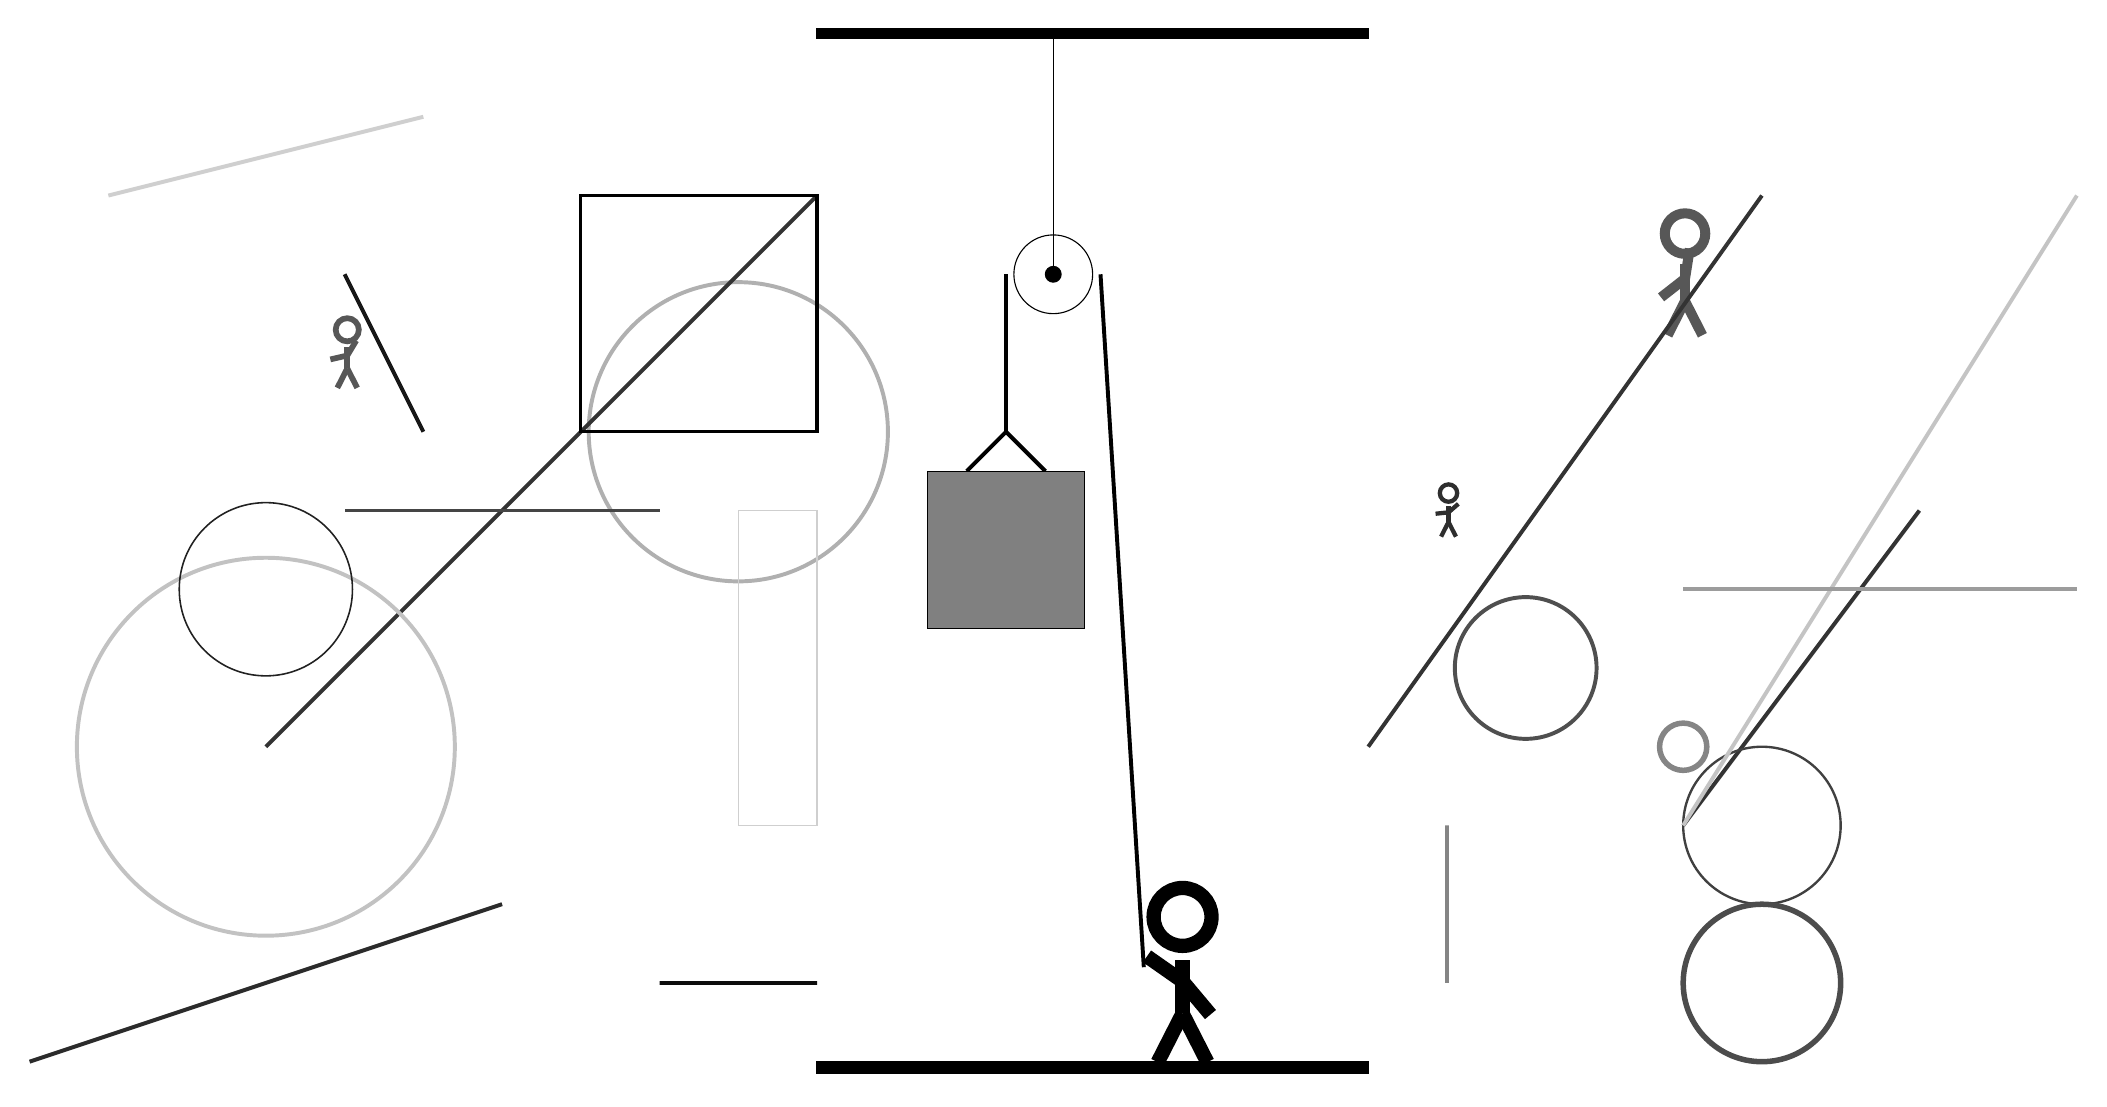
\begin{tikzpicture}
		%%%%% START %%%%%
		
		\draw[fill=black] (-2, 10) rectangle (5, 10.125);
		
		\draw (1, 7) circle (0.5);
		\draw[fill=black] (1, 7) circle (0.1);
		\draw (1, 10) -- (1, 7);
		
		\draw [line width=0.5mm, color=black!31](-3, 5) circle (1.9);
		
		\draw[line width=0.5mm, color=black!80](-2, 8) -- (-9, 1);
		\draw[line width=0.5mm, color=black!19](-7, 9) -- (-11, 8);
		\draw[line width=0.5mm, color=black!91](-7, 5) -- (-8, 7);
		\draw[line width=0.4mm, color=black!100] (-2, 5) rectangle (-5, 8);
		\draw [line width=0.7mm, color=black!48](9, 1) circle (0.3);
		\draw [line width=0.5mm, color=black!69](7, 2) circle (0.9);
		
		\draw [line width=0.5mm, color=black!24](-9, 1) circle (2.4);
		\node[line width=0.6mm, color=black!82] at (6, 4) {\Strichmaxerl[3][6][41]};
		
		\draw[line width=0.5mm, color=black!80](9, 0) -- (12, 4);
		\draw [line width=0.3mm, color=black!75](10, 0) circle (1.0);
		\node[line width=0.6mm, color=black!66] at (-8, 6) {\Strichmaxerl[4][13][59]};
		\node[line width=0.7mm, color=black!66] at (9, 7) {\Strichmaxerl[7][38][81]};
		
		\draw[line width=0.6mm, color=black!95] (-2, -2) rectangle (-4, -2);
		\draw[line width=0.5mm, color=black!73](-4, 4) -- (-8, 4);
		\draw[line width=0.5mm, color=black!23](9, 0) -- (14, 8);
		
		\draw [line width=0.7mm, color=black!70](10, -2) circle (1.0);
		\draw[line width=0.5mm, color=black!80](5, 1) -- (10, 8);
		\draw[line width=0.4mm, color=black!48] (6, -2) rectangle (6, 0);
		\draw[line width=0.2mm, color=black!19] (-3, 4) rectangle (-2, 0);
		\draw[line width=0.5mm, color=black!83](-6, -1) -- (-12, -3);
		
		\draw [line width=0.2mm, color=black!87](-9, 3) circle (1.1);
		
		\draw[line width=0.5mm, color=black!39](9, 3) -- (14, 3);
		
		\draw[line width=0.5mm] (-0.1, 4.5) -- (0.4, 5.0) -- (0.9, 4.5);
		\draw[fill=black!50] (-0.6, 4.5) rectangle (1.4, 2.5);
		
		\draw[line width=0.5mm] (0.4, 7) -- (0.4, 5.0);
		\centerarc[line width=0.5mm](1, 7)(0:180:0.6);
		\draw[line width=0.5mm](1.6, 7) -- (2.15, -1.8);
		
		\node at (2.6, -1.9) {\Strichmaxerl[10][-35][-50]};
		
		\draw[fill=black] (-2, -3) rectangle (5, -3.15);
		
		%%%%% END %%%%%
	\end{tikzpicture}
\end{document}